Uma estação meteorológica é um equipamento, assemelhado a uma torre, que possui diversos tipos de instrumentos necessários aos estudos do tempo e do clima. A leitura desses instrumentos permite conhecer o estado presente da atmosfera. Estas estações podem ser de dois tipos: convencionais e automáticas. O primeiro tipo de estação necessita da ação humana para completar seu processo de aferição e coleta dos dados. Já o segundo tipo de estação, as estações meteorológicas automáticas, não depende de uma pessoa para a realização de suas funções \cite{Vianello:Livro}.

Uma estação meteorológica automática é uma torre de observação, constituida por um conjunto de sensores eletrônicos automáticos de alta precisão, instalada no interior de um cercado, rigorosamente construída e operando segundo padrões internacionais. Inicialmente as estações automatáticas tinham como objetivo principal complementar a rede básica de estações convencionais, cobrindo regiões de difícil acesso, suprindo a falta de pessoal especializado para complementar o proceso de medições. Porém, considerando a possiblidade de observações em diferentes horários e o alto grau de confiabilidade dos dados obtidos, estas têm substituído significativamente as estações convencionais  \cite{Vianello:Livro}.

Dentre diversas outras atividades, o LabInstru administra uma estação meteorológica automática localizada nas dependências da Escola Superior de Tecnologia, ilustrada na Figura \ref{fig:ema}. Esta encontra-se em um cercado construído conforme as normas da Organização Meteorológica Mundial, com dimensões de $10 \times 15$ metros quadrados, com alambrado de $1,5$ metros pintado na cor branca. No centro deste cercado encontra-se um tripé de Campbell com $3$ metros de altura, o qual serve de suporte para diversos sensores instalados ao longo de sua extensão, bem como para os sistemas de aquisição e armazenamento dos dados, alimentação, e transmissão dos dados \cite{Labinstru:EST}.

\newpage

\begin{figure}
\begin{minipage}{\textwidth}
  \begin{minipage}[b]{0.59\textwidth}
    \centering
    	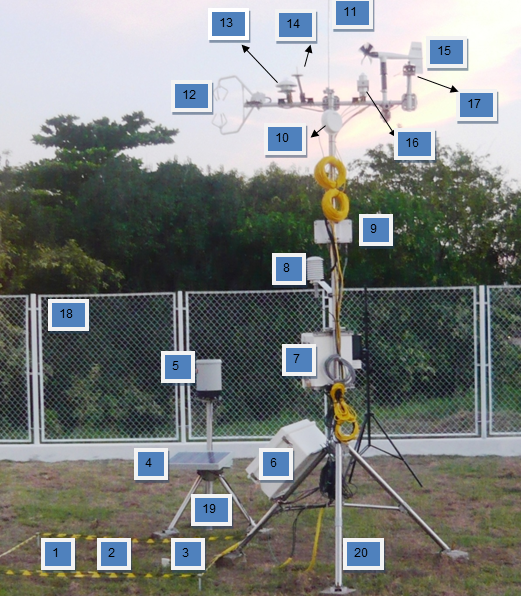
\includegraphics[width=\textwidth]{./img/ema5.png}
  \end{minipage}
  \hfill
  \begin{minipage}[b]{0.39\textwidth}
    \centering
		\begin{footnotesize}
		\begin{tabular}{cc}
		\toprule
		Item & Descrição\\
		\midrule
		1 & Reflectômetro \\
		2 & Placa de fluxo de calor no solo\\
		3 & Perfilador de temperatura no solo\\
		4 & Painel solar\\
		5 & Pluviômetro \\
		6 & Ver Figura \ref{fig:ema2}\\
		7 & Ver Figura \ref{fig:ema3}\\
		8 & Termohigrômetro\\
		9 & Caixa do sônico\\
		10 & Antena de transmissão de dados\\
		11 & Para-raio\\
		12 & Anemômetro sônico\\
		13 & Albedômetro \\
		14 & Saldo radiômetro (NR-LITE)\\
		15 & Anemômetro\\
		16 & Saldo radiômetro (CNR1)\\
		17 & Radiômetro\\
		18 & Cercado \\
		19 & Tripé de 1 metro \\
		20 & Tripé de 3 metros\\
		\bottomrule
		\end{tabular}
	\end{footnotesize}
    \end{minipage}
  \end{minipage}
	\caption{Estação meteorológica automática da EST e descrição dos seus componentes. Fonte: \cite{Labinstru:EST}.}\label{fig:ema}
\end{figure}

Próximo ao tripé da haste, encontram-se instalados os sensores para monitoramento das condições do solo. São eles:
\begin{enumerate}
	\item Reflectômetro para medida de conteúdo de água no solo (CS 616 - Campbell);
	\item Placa de fluxo de calor no solo (HFP01 - Hukseflux) instaladas em 5cm;
	\item Perfilador de temperatura no solo (STP01 - Hukseflux) medindo a temperatura nas profundidades de 2, 5,   10, 20 e 50 cm;
\end{enumerate}

Ao longo da haste do tripé encontram-se os seguintes sensores:
\begin{enumerate}
	\item Anemômetro sônico (CSAT3 - Campbell) para gerar medidas das componentes ortogonais do vento e temperatura virtual do ar;
	\item Anemômetro (05106 - Young) para medida da direção e velocidade do vento;
	\item Barômetro (CS106 - Vaisala) para medir a pressão atmosférica;
	\item Termohigrômetro (HMP45C - Vaisala) para medir temperatura e umidade do ar;
	\item Saldo radiômetro (NR-LITE – Kipp \& Zonen) para a medida do saldo de radiação;
	\item Saldo radiômetro (CNR1 - Kipp \& Zonen) para medidas da radiação solar incidente e refletida, e radiação terrestre e atmosférica emitidas;
	\item Radiômetro PAR (PAR LITE - Kipp \& Zonen) para a medida da componente fotossinteticamente ativa da radiação solar;
	\item Albedômetro (CMA11 - Kipp \& Zonnen) para medidas das radiações solar incidente e refletida \cite{Labinstru:EST}.
\end{enumerate}

Ao lado do tripé de $3$m, um segundo tripé de $1$ metro de altura serve de suporte para um pluviômetro (TB4 - Hydrological Services), que totaliza a precipitação, e para o painel solar. Há também a caixa do sônico, a antena de transmissão dos dados e um pára-raios. Uma caixa de poliéster reforçada com fibra de vidro, abriga o sistema de aquisição dos dados (\emph{datalogger}), barômetro e interface para gravação dos dados (NL 115, Campbell) \cite{Labinstru:EST}, conforme ilustrado detalhadamente na Figura \ref{fig:ema2}. Uma outra caixa abriga duas baterias, o controlador de carga e um roteador, conforme mostra a Figura \ref{fig:ema3}.

\begin{figure}[h!]
	\centering
	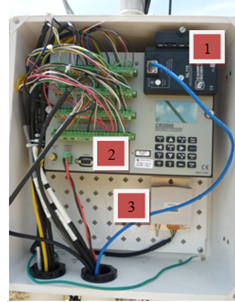
\includegraphics[width=0.3\textwidth]{./img/ema6.png}
	\caption{Detalhamento do item 6 da Figura \ref{fig:ema}. O item 1 indica a interface para gravação dos dados, o item 2 indica o \emph{datalogger} e o item 3 indica o barômetro. Fonte: \cite{Labinstru:EST}} \label{fig:ema2}
\end{figure}

\begin{figure}[h!]
	\centering
	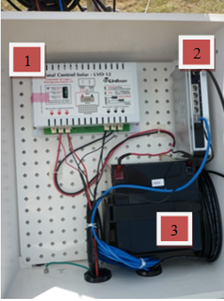
\includegraphics[width=0.3\textwidth]{./img/ema7.png}
	\caption{Detalhamento do item 7 da Figura  \ref{fig:ema}, referente à transmissão de dados. O item 1 consiste em um regulador de voltagem, o item 2 em um roteador e o item 3 em uma bateria. Fonte: \cite{Labinstru:EST}} \label{fig:ema3}
\end{figure}

Todos os sinais dos sensores, bem como a voltagem da bateria, são medidos por um sistema de aquisição e armazenamento de dados (\emph{datalogger}), programado para realizar leitura a cada segundo e gravar os dados em um certo intervalo de tempo. A transmissão dos dados pode ser realizada de duas formas: por meio da gravação dos dados em um cartão removível de $2$ GB ou via conexão wireless utilizando o protocolo TCP/IP entre o \emph{datalogger} CR3000 e um computador remoto, contendo um programa específico para a correta transmissão do dados. A Figura \ref{fig:ema4} exemplifica o passo a passo da transmissão.

\begin{figure}[H]
	\centering
	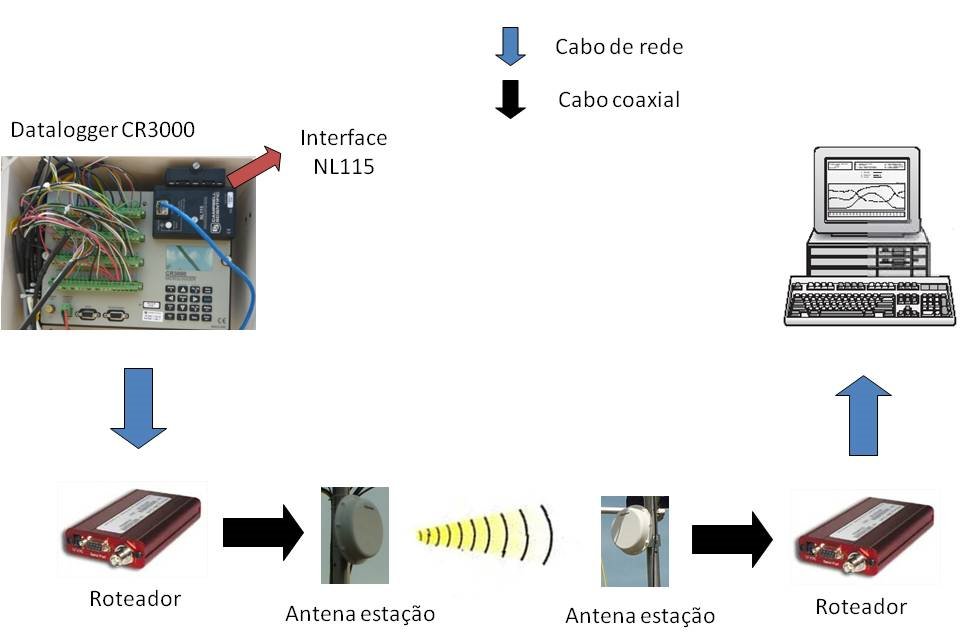
\includegraphics[width=1\textwidth]{./img/ema4.png}
	\caption{Esquema de transmissão dos dados da estação meteorológica. Fonte: \cite{Labinstru:EST}} \label{fig:ema4}
\end{figure}

Após a transmissão, a equipe do LabInstru passa a ter acesso aos dados capturados pela estação.  Além das informações meteorológicas, a estação também fornece dados de controle, tais como carga da bateria, tempo estimado de funcionamento, etc. Todos os dados produzidos são persistidos em um arquivo-texto de maneira serializada a intervalos de tempo fixos e pré-determinados de dez minutos. O arquivo, embora possua uma estrutura textual, assemelha-se a uma ``tabela'' como maneira de organizar os dados. A Figura \ref{fig:exemploBaixa1} ilustra um trecho deste arquivo. As linhas 1-8 mostram o cabeçalho do arquivo, que descreve quais variáveis serão persistidas a partir deste momento pela estação meteorológica. As linhas 9-11 e 12-14 exemplificam dois registros de dados da estação meteorológica feitos no dia $05$ de Fevereiro de $2014$ às 09h40min e às 09h50min, respectivamente.

Atualmente, os responsáveis pelo LabInstru abrem este arquivo de maneira manual e, utilizando softwares editores de texto e de planilhas, geram sumários, estatíticas, gráficos, dentre outros. Como pode ser visto, explorar manualmente estes arquivos, especialmente considerando um longo período de tempo, é um trabalho difícil e demorado. A minimização destas dificuldades é uma das motivações para a realização deste trabalho.

\begin{figure}[H]
\centering
\begin{scriptsize}
\fbox{
    \begin{minipage}{1\textwidth}
	    \internallinenumbers
	    `TIMESTAMP', `RECORD', `batt\_volt\_Min', `PTemp', `NRLite\_Avg', `CM3Up\_Avg', `CM3Dn\_Avg', `CG3UpCorr\_Avg', `CG3DnCorr\_Avg', `CNR1TC\_Avg', `CMA11Up\_Avg', `CMA11Dn\_Avg', `LI190S\_Avg', `VW\_Avg', `HFP01\_Avg', `STP01\_50cm\_Avg', `STP01\_20cm\_Avg',  `STP01\_10cm\_Avg', `STP01\_5cm\_Avg', `STP01\_2cm\_Avg', `CS106\_Avg', `HMP45C\_Temp\_Avg', `HMP45C\_RH\_Avg', `WindSpeed', `WindDirection', `TB4\_Tot', `TS', `RN', `', `', `W/m2', `W/m2', `W/m2', `W/m2', `W/m2', `deg\_C', `W/m2', `W/m2', `umol/mol', `\%', `W/m2', `deg\_C', `deg\_C', `deg\_C', `deg\_C', `deg\_C', `hPa', `dec\_C', `\%', `m/s', `Deg', `mm', `', `', `Min', `Smp', `Avg', `Avg', `Avg', `Avg', `Avg', `Avg', `Avg', `Avg', `Avg', `Avg', `Avg', `Avg', `Avg', `Avg', `Avg', `Avg', `Avg', `Avg', `Avg', `WVc:Averaged\_Value', `WVc:Averaged\_Value', `Tot'\\
`2014-02-05 09:40:00',  118726,  13.23,  28.78, 233.1908, 359.7406, 60.10703, 1249.177, 1290.342, 115.3246, 363.9763, 65.63671, 448.9503, 0.2546729, `NAN',  29.45563, 28.85126, 28.97074, 29.36523, 29.92229, 1009.477, 27.5499, 79.00884, 0.7635838, 103.2079, 0\\
`2014-02-05 09:50:00',  118727, 13.24, 29.03, 218.5598, 342.636, 56.87075, 1259.051, 1300.909, 116.1448, 346.5667, 62.29135, 430.326, 0.2546285, `NAN',  29.45018, 28.87249, 29.0521, 29.47018, 29.96688, 1009.529, 27.53578, 78.62649, 0.8266301, 113.4006, 0
    \end{minipage}
}
\end{scriptsize}
\caption{Exemplo de um trecho dos dados encontrados no arquivo produzido pela estação meteorológica.} \label{fig:exemploBaixa1}
\end{figure}

\newpage